\begin{figure*}[ht]
\centering
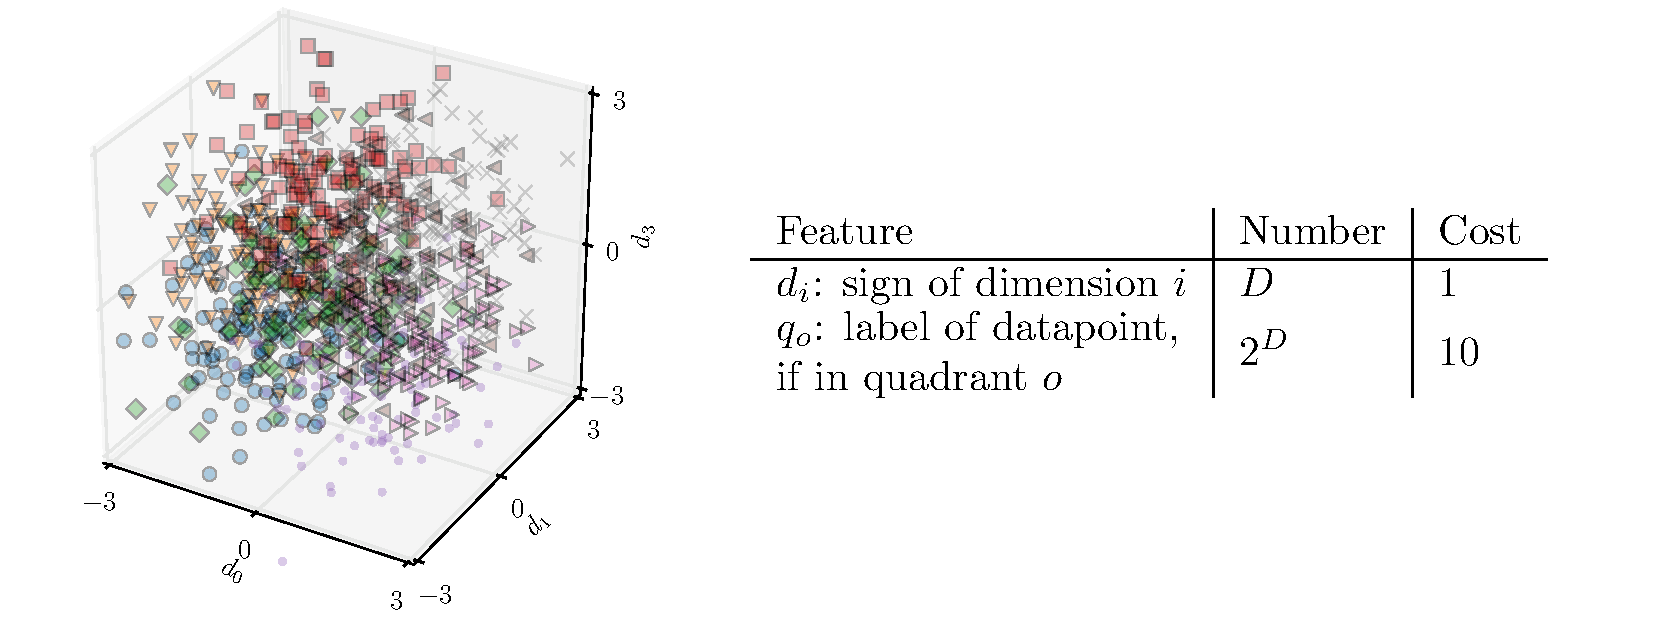
\includegraphics[width=\linewidth]{../../figures/synthetic_explanation.pdf}
\caption[Setup of the synthetic example.]{
See text for explanation.
}\label{fig:synthetic_setup}
\end{figure*}


\begin{figure*}[ht]
\centering
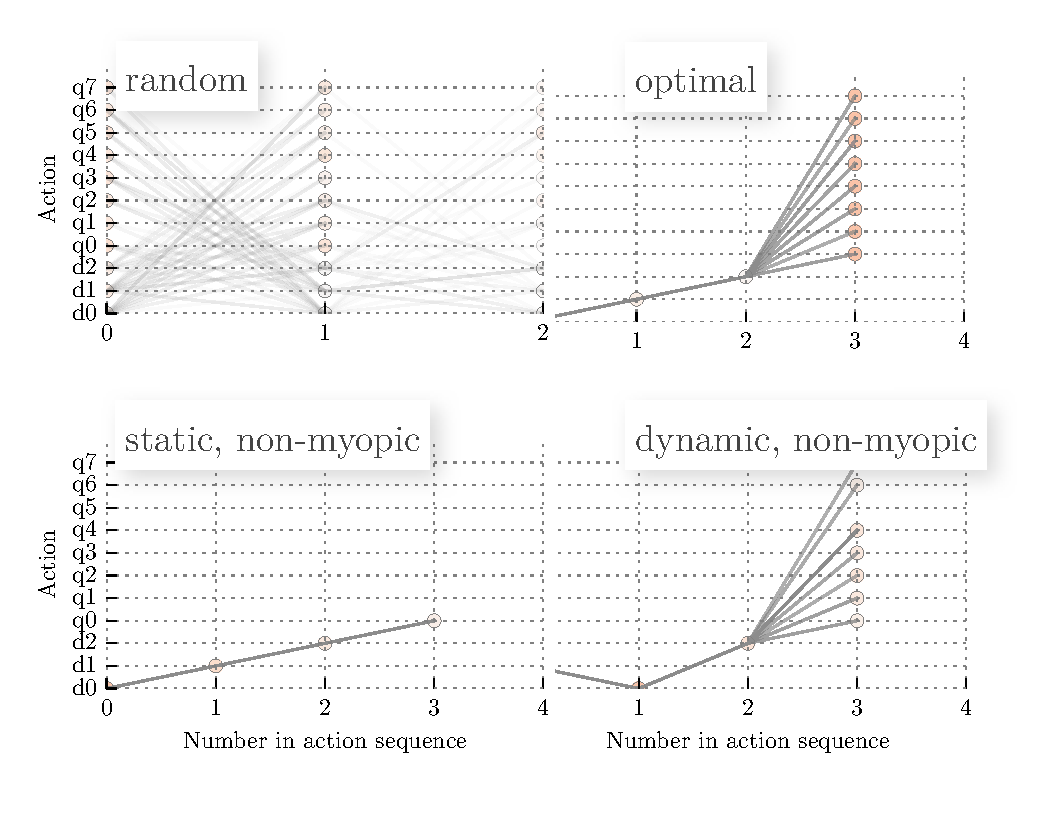
\includegraphics[width=\linewidth]{../../figures/synthetic_trajectories.pdf}\\
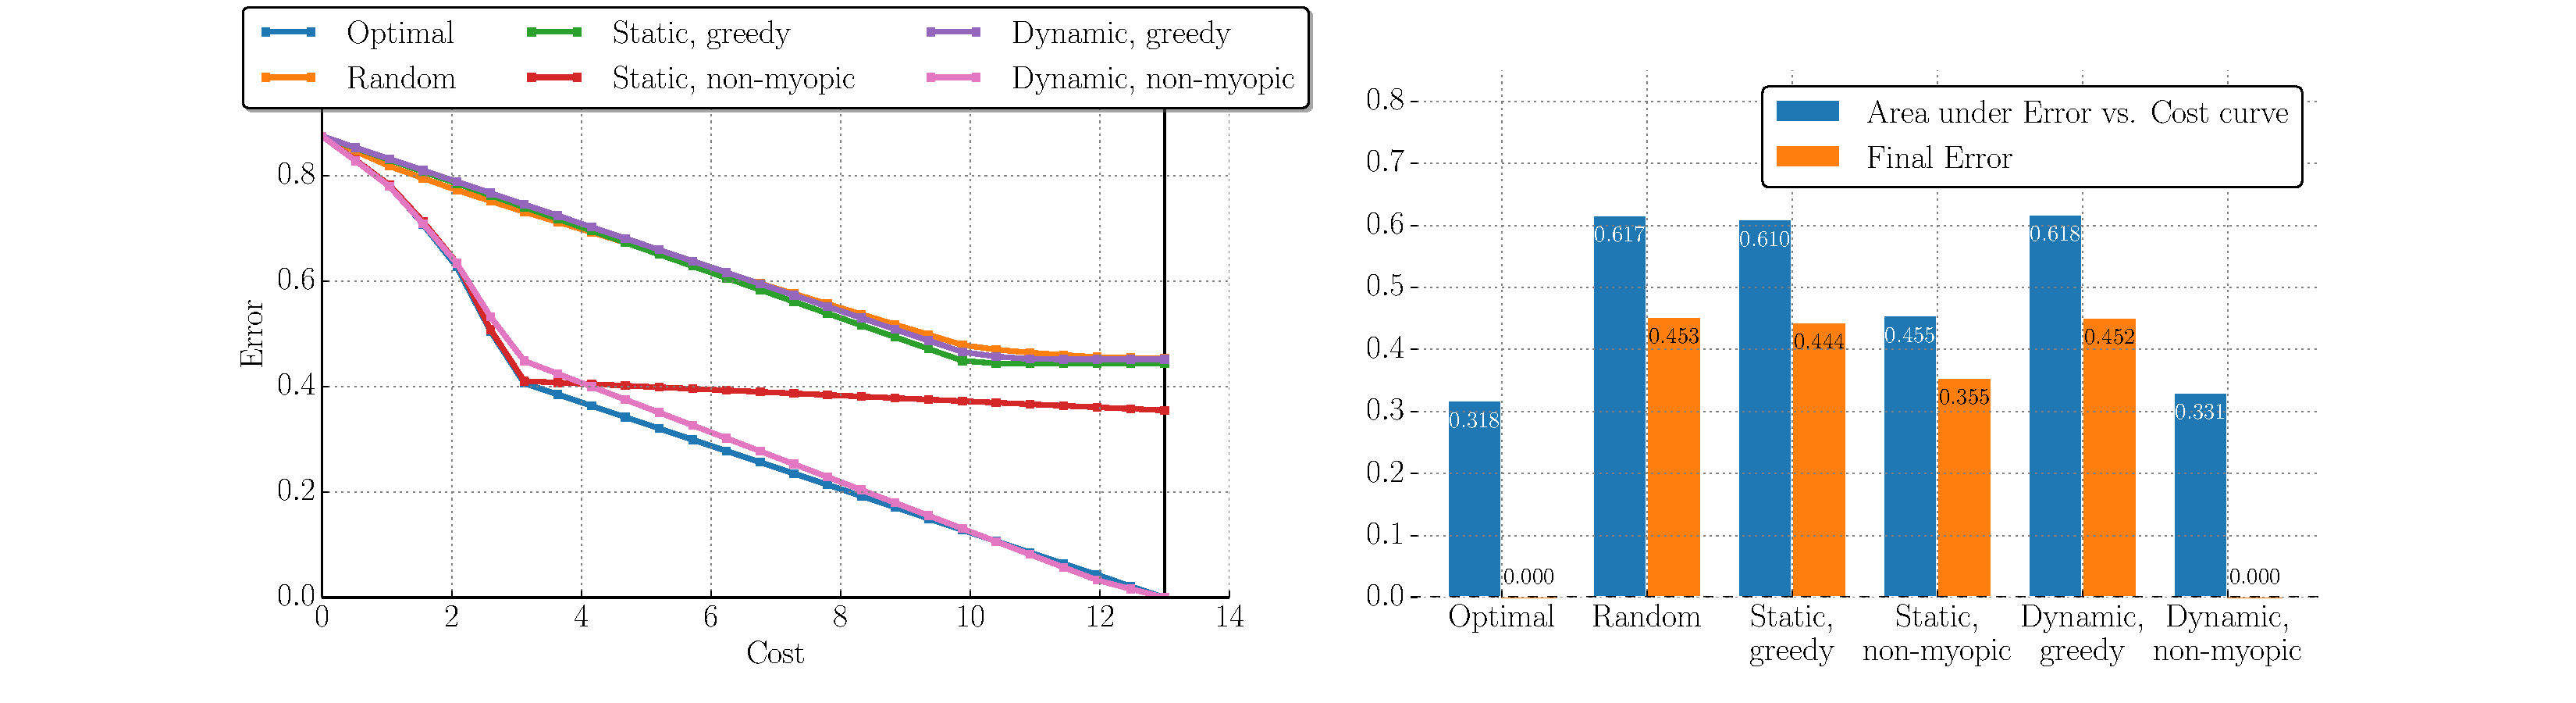
\includegraphics[width=\linewidth]{../../figures/apr11_assembly/synthetic_orthants_D3_False_N16000_Nt4000_13.pdf}
\caption[Evaluation of the classification approach on the synthetic example.]{
Evaluation on the synthetic example (best viewed in color).
The sample feature trajectories of different policies at top: the opacity of the edges corresponds to their prevalence during policy execution; the opacity of the nodes corresponds to the amount of reward obtained in that state.
Note that the \emph{static, non-myopic} policy correctly learns to select the cheap features first, but is not able to correctly branch, while our \emph{dynamic, non-myopic} approach finds the optimal strategy.
The plots in the bottom half give the error vs. cost numbers.
}\label{fig:synthetic_results}
\end{figure*}
